% !TEX program = lualatex
\documentclass[aspectratio=43,professionalfonts,handout]{beamer}
\usepackage{beamer_template}

\newcommand{\LectureNum}{15}
\newcommand{\LectureTitle}{前期復習}
\newcommand{\TextPages}{p.\,72-100}
\newcommand{\NextTopic}{}
\newcommand{\NextPages}{対応なし}
\newcommand{\CourseName}{基礎数学B}
\renewcommand{\TermName}{前期}

\begin{document}

% -----------------------------------------------
% スライド1: 表紙＋目標＋用語・定義
% -----------------------------------------------
\begin{frame}{\CourseName\quad 第\LectureNum 回「\LectureTitle 」}
  {\small \TermName\quad \TeacherName\quad ／\quad 教科書 \TextPages\quad
  \textbf{目標}：前期全範囲（3章）を総復習し、定期試験に備える}

  \begin{block}{用語・定義}
  \begin{description}[labelwidth=5.5em]
    \item[\kw{3章1節（2次関数）}] ~
    \item[\kw{3章2節（いろいろな関数）}] ~
    \item[\kw{共通テーマ}] ~
  \end{description}
  \end{block}
\end{frame}

% -----------------------------------------------
% スライド2: 公式・性質
% -----------------------------------------------
\begin{frame}{公式・性質}
  \begin{block}{}
  \begin{itemize}
    \item 前期全範囲の重要公式一覧
  \end{itemize}
  \end{block}
\end{frame}

% -----------------------------------------------
% スライド3: 図・グラフ（TikZコードを手動追加）
% -----------------------------------------------
\begin{frame}{図・グラフ}
  \centering
  % TODO: 標準形・最大最小・判別式・2次不等式 各1問
  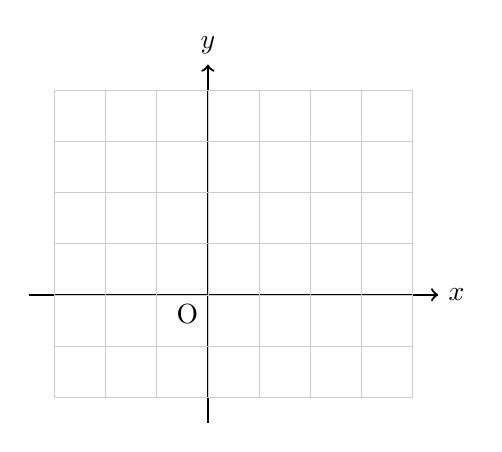
\begin{tikzpicture}[scale=0.65]
    \draw[->,thick] (-3.5,0) -- (4.5,0) node[right]{$x$};
    \draw[->,thick] (0,-2.5) -- (0,4.5) node[above]{$y$};
    \node[below left] at (0,0) {O};
    \draw[gray!40, very thin] (-3,-2) grid (4,4);
    % ここにグラフを描画
  \end{tikzpicture}
\end{frame}

% -----------------------------------------------
% スライド4: 確認問題2（いろいろな関数）
% -----------------------------------------------
\begin{frame}{確認問題2（いろいろな関数）}
\end{frame}

% -----------------------------------------------
% スライド5: 解答確認
% -----------------------------------------------
\begin{frame}{解答確認}
\end{frame}

% -----------------------------------------------
% まとめ
% -----------------------------------------------
\begin{frame}{まとめ}
  \begin{itemize}
    \item 2次関数：標準形・最大最小・判別式・2次不等式
    \item いろいろな関数：べき・分数・無理・逆関数
    \item 共通のキーワード：定義域・値域・グラフ・平行移動・対称移動
  \end{itemize}
\end{frame}

\end{document}
